\documentclass[tikz,border=5pt]{standalone}
\usepackage{tikz}
\usetikzlibrary{arrows.meta,positioning,calc}
\definecolor{nebula}{HTML}{6366F1}
\definecolor{spark}{HTML}{14B8A6}
\definecolor{ink}{HTML}{334155}
\begin{document}
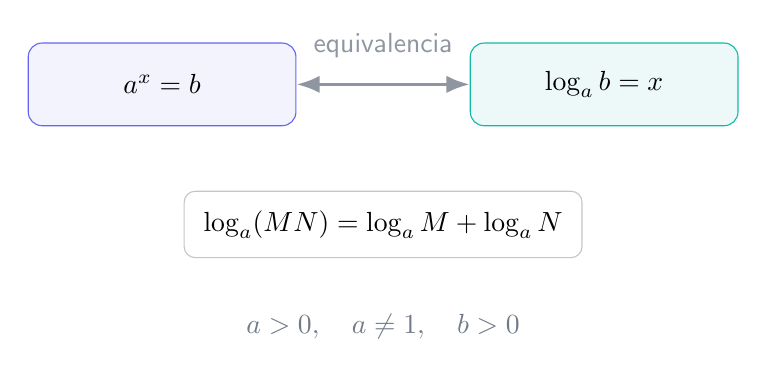
\begin{tikzpicture}[font=\sffamily,>=Latex,node distance=2.2cm]
  \node[draw=nebula,rounded corners=5pt,fill=nebula!8,minimum width=3.4cm,minimum height=1.05cm] (exp)
    {$a^x=b$};
  \node[draw=spark,rounded corners=5pt,fill=spark!8,minimum width=3.4cm,minimum height=1.05cm,right=of exp] (log)
    {$\log_a b=x$};
  \draw[<->,very thick,ink!55] (exp)--(log) node[midway,above=7pt,fill=white,inner sep=2pt] {equivalencia};
  \node[draw=ink!30,rounded corners=4pt,fill=white,inner sep=7pt,below=1.35cm of $(exp)!0.5!(log)$]
    {$\log_a(MN)=\log_aM+\log_aN$};
  \node[text=ink!70,below=2.8cm of $(exp)!0.5!(log)$]
    {$a>0,\quad a\neq1,\quad b>0$};
\end{tikzpicture}
\end{document}
